\chapter{Модель гистерезисного микроансамбля} \label{chapter:neuron}

В главе даётся формальное определение модели нейрона в виде системы обыкновенных дифференциальных уравнений, а так же определяется понятие микроансамбля --- сильно связного объединения нейронов. Анализируются точки равновесия и проводится бифуркационный анализ. В результате, определяются основные понятия и характерные свойства, связанные с предлагаемой моделью, а так же моделируются типичные сценарии функционирования простой модели микроансамбля. При этом рассматривается применение двух различных функций активации: \textit{оригинальной} и \textit{сигмоидальной}. 

Кроме того, для апробации предлагаемой модели микроансамбля на её основе реализуются две \acr{NN}, первая из которых решает задачу анализа независимых компонент, а вторая моделирует детерминированный конечный автомат. 


%==============================================================================
%                          Формальное определение модели
%==============================================================================
\section{Формальное определение} \label{section:neuron_model}

Основой для рассматриваемой в данной главе модели нейрона послужила монография~\cite{EmelyanovYaroslavsky1990}, в которой описан подход к построению искусственной \acr{NN}, потенциально обладающей интеллектуальными свойствами и названной автором \textit{индуктивным автоматом}. Особенность работы заключается в том, что автор предлагает оригинальную модель нейрона и показывает через численные и умозрительные эксперименты, что благодаря ряду локальных свойств совокупность нейронов способна демонстрировать нетривиальное поведение. Однако предложенная нейросетевая модель носит ярко выраженный незаконченный характер и кроме того, преследует целью биологическую правдоподобность, что так же отразилось на сложности модели.

Данная диссертационная работа направлена на получение потенциальной прикладной значимости, в частности, при решении задачи контекстно-зависимого распознавания образов. Поэтому предложенный в работе~\cite{EmelyanovYaroslavsky1990} подход был в значительной мере переосмыслен и в результате была выработана собственная нейросетевая модель: она не содержит биологически обоснованных и стохастических элементов, а так же в противоположность \textit{Integrate-And-Fire} типу модели, где подразумевается моделирование на уровне отдельных импульсов нейрона с частотно-фазовым кодированием информации, является более классической \textit{Firing-Rate}  моделью~\cite{Dayan2001}, в которой выходным параметром нейрона является \socalled частота --- усреднённая по времени частота генерации импульсов. И хотя первый тип обладает более разнообразной поведенческой динамикой и информационной ёмкостью~\cite{Izhikevich2006}, практическое применение этого типа моделей сопряжено с рядом проблем, начиная со сложностей в их анализе и заканчивая вычислительной дороговизной.

Таким образом, формальная модель нейрона приобрела следующий вид:
\begin{equation}
	\label{eq:full_single_neuron_model}
    \begin{cases}
	    d\scalar{u}/d\scalar{t} &= \vector{w}^{\top} \vector{x} - \scalar{p} - \mu \scalar{u}, \\
        \scalar{y}              &= f\left( \scalar{u}, \theta \right), \\
    \end{cases}
\end{equation}
где $\scalar{u} \in \specialset{R}$ --- потенциал нейрона, $\vector{x} \in \specialset{R}^{M}$ -- входной вектор нейрона (входной сигнал), $\vector{w} \in \specialset{R}^{M}$ --- вектор весовых коэффициентов нейрона,  $\scalar{p}$ --- внутренний порог нейрона, $\mu \in \left(0;1\right)$ --- константа, характеризующая скорость убывания потенциала нейрона (константа диссипации), $\scalar{y} \in \left[0;1\right]$ --- частота нейрона (выходной сигнал), $\theta \in \specialset{R}^{+}$ --- управляющий параметр сети, который будет рассмотрен более подробно в следующих главах. 

Для удобства дальнейшего изложения мы применим приём, который часто используется в области нейросетевого моделирования, а именно: положим, что $\vectoritem{x}{0}$ в любой момент времени равно $1$ и $\vectoritem{w}{0}$ равно $-\scalar{p}$, тогда выражение~\eqref{eq:full_single_neuron_model} можно записать в более компактной эквивалентной форме:
\begin{equation}
    \label{eq:single_neuron_model}
    \begin{cases}
    d\scalar{u}/d\scalar{t} &= \vector{w}^{\top} \vector{x} - \mu \scalar{u}, \\
    \scalar{y}              &= f\left( \scalar{u}, \theta \right), \\
    \end{cases}
\end{equation}
которая будет использована далее наравне с выражением~\eqref{eq:full_single_neuron_model}.

Функция активации $f: \specialset{R} \to \left[0;1\right]$ преобразует потенциал нейрона $\scalar{u}$ в его выходную частоту $\scalar{y}$ как:
\begin{equation}
    \label{eq:activation_function}
    f\left( \scalar{u}, \theta \right) = g\left( \tilde{\scalar{u}} \right), 
\end{equation}
где $\tilde{\scalar{u}} = \scalar{u} / \theta$, а в качестве $g$ в главе будут рассмотрены две функции, изображённые \onfigure~\ref{fig:model_activation_functions} (далее функции $f$ и $g$ будут в равной степени называться функциями активации):

\IncludeFigure{model_activation_functions}{Вид оригинальной $g_{s}$ и сигмоидальной $g_{\sigma}$ функций активации.}

\begin{itemize}
	\item \textit{Оригинальная} функция $g_{s}$, полученная на основе функции динамического порога $\text{П}^\text{Д}$ из работы~\cite{EmelyanovYaroslavsky1990}, но отличающаяся от неё в виду того, что аргументом функции  $\text{П}^\text{Д}$ является межимпульсный интервал и, что важнее, она не была задана автором аналитически (подробнее вывод функции $g_{s}$ рассмотрен \inappendix~\ref{appendix:activation_function}):
		\begin{equation}
            \label{eq:activation_function_original}
            g_{s}(\tilde{\scalar{u}}) = 
            \begin{cases}
                0                                                                                               &, \tilde{\scalar{u}} < u_{01} \\
                0,1935 + \dfrac{1}{120} \ln\left( \dfrac{\tilde{\scalar{u}}}{2,6 - \tilde{\scalar{u}}} \right)  &, u_{01} \le \tilde{\scalar{u}} \le u_{12} \\
                1 - \dfrac{z_{12}}{\tilde{\scalar{u}} - k_{12}}                                                   &, \tilde{\scalar{u}} > u_{12} \\
            \end{cases}
		\end{equation}
        где значения коэффициентов равны ($\sigma$ --- логистическая функция):
        \begin{align*}
            &z_{12} = 177,84 \cdot \sigma\left(6,18\right) \cdot \left(1 - \sigma\left(6,18\right)\right) \approx 0,37, \\
            &k_{12} = 2,6 \cdot \sigma\left(6,18\right) - z_{12} / 0,755 \approx 2,11, \\
            &u_{01} = 2,6 \cdot \sigma\left(-23,22\right) \approx 0, \\
            &u_{12} = 2,6 \cdot \sigma\left(6,18\right) \approx 2,6.
        \end{align*}
	\item \textit{Сигмоидальная} функция $g_{\sigma}$, которая получила широкое распространение в области нейронных сетей, нечёткой логики и \other, в виде:
		\begin{equation}
            \label{eq:activation_function_sigma}
			g_{\sigma}(\tilde{\scalar{u}}) = \dfrac{1}{1 + e^{\displaystyle -(\tilde{\scalar{u}} - 3)}}.
		\end{equation}
\end{itemize}


\begin{Definition*}
    Определим \textit{микроансамбль} в виде математической структуры $A = \left\{ \customset{N}, \matrix{V} \right\}$, где $\customset{N} = \left\{ n_{i} \right\}_{i=1}^{N} $ --- множество нейронов, составляющих микроансамбль, и $\matrix{V}_{N \times N}$ --- матрица, задающая топологию и коэффициенты связей между нейронами микроансамбля. При этом размер множества $\customset{N}$ и значение матрицы $\matrix{V}$ фиксированы, \ie не меняются в процессе обучения и функционирования сети, и выбираются заранее, исходя из требуемых вычислительных свойств микроансамбля как целостной вычислительной единицы \acr{NN}.
\end{Definition*}

Основываясь на выражении~\eqref{eq:single_neuron_model}, динамика микроансамбля может быть описана следующим образом:
\begin{equation}
    \label{eq:microensemble_model}
    \begin{cases}
        d\vector{u}/d\scalar{t} &= \matrix{V}^{\top} \vector{y} + \matrix{W}^{\top} \vector{x} - \mu \vector{u}, \\
        \vector{y}              &= f\left( \vector{u}, \theta \right), \\
    \end{cases}
\end{equation}
где все параметры и переменные имеют тот же смысл, что и в выражении~\eqref{eq:single_neuron_model}, но записанные в векторно-матричной форме, а матрица $\matrix{W}_{M \times N} = \left[ \vector{w}_{1} \ldots \vector{w}_{N} \right]$, составленная из векторов-столбцов $\vector{w}_{i}$, отражает связи входного вектора $\vector{x}$ со всеми нейронами микроансамбля.

Для дальнейшего анализа и выявления характерных свойств модели микроансамбля, которые затем позволят оценить её с точки зрения вычислительного элемента \acr{NN}, введём понятие простого микроансамбля.
\begin{Definition*}
    Будем называть микроансамбль $A$ \textit{простым микроансамблем}, если выполнены следующие условия:
    \begin{itemize}
        \item все нейроны микроансамбля соединены друг с другом связями весом $\omega$, \ie: $\matrix{V}_{N\!\times\!N} = \omega \cdot \left( \matrix{J}_{N\!\times\!N} - \matrix{I}_{N} \right)$, где матрицы $\matrix{J}$ и $\matrix{I}$  --- матрица единиц и единичная матрица соответственно;
        \item все нейроны микроансамбля имеют одинаковые связи с входным вектором $\vector{x}$, \ie: $\forall\ i \in \overline{1,N}\ \vector{w}_{i} = \vector{w}$;
        \item начальные условия для всех нейронов микроансамбля совпадают, \ie: \par $\vector{u}|_{t=0} = \scalar{u}^{0} \cdot \matrix{J}_{N\!\times\!1}$, где $\scalar{u}^{0}$ --- начальное значение потенциала.
    \end{itemize}
\end{Definition*}

В этом случае можно говорить об эквивалентности всех нейронов микроансамбля, а значит всё множество нейронов $\customset{N}$ может быть представленно в виде одного гипер-нейрона с рекуррентной связью на себя, как показано \onfigure~\ref{fig:model_simple_microensemble}. Выражение~\eqref{eq:microensemble_model} при этом примет более простую форму:
\begin{equation}
    \label{eq:simple_microensemble_model}
    \begin{cases}
    d\scalar{u}/d\scalar{t} &= \alpha \scalar{y} + \vector{w}^{\top} \vector{x} - \mu \scalar{u}, \\
    \scalar{y}              &= f\left( \scalar{u}, \theta \right), \\
    \end{cases}
\end{equation}
где параметр $\alpha = \omega \cdot \left( N - 1 \right)$ --- весовой коэффициент рекуррентной связи, который по смыслу отражает связность нейронов микроансамбля. Выражение~\eqref{eq:simple_microensemble_model} так же можно представить в виде, характерном при описании рекуррентных нейронов в нейродинамике~\cite{Haykin2008}:
\begin{equation}
    \nonumber
    d\scalar{u}/d\scalar{t} = \alpha f\left( \scalar{u}, \theta \right) + \vector{w}^{\top} \vector{x} - \mu \scalar{u}.
\end{equation}
Однако запись в виде системы более удобна в том смысле, что явно содержит выходную переменную $y$.

\IncludeFigure{model_simple_microensemble}{Приведение простого микроансамбля с 3-мя нейронами к виду эквивалентного гипер-нейрона с рекуррентной связью $\alpha$ на себя.}

Стоит отметить, что в работе~\cite{Pchelkin2003} исследовалась похожая на систему~\eqref{eq:simple_microensemble_model} модель нейронного ансамбля, которая так же была основана на развитии идей индуктивного автомата~\cite{EmelyanovYaroslavsky1990}. Однако автор, во-первых, не учитывал внешнее влияние на нейроны (слагаемое $\vector{w}^{\top} \vector{x}$), и во-вторых, был сосредоточен на конкретной проблеме, а именно на связи поведения модели с \socalled оптимальной частотой --- основополагающим параметром модели индуктивного автомата, который в явном виде отсутствует в рассматриваемой нами модели.


%==============================================================================
%                   Точки равновесия и бифуркационный анализ
%==============================================================================
\section{Точки равновесия и бифуркационный анализ} \label{section:neuron_equilibrium}

Для удобства дальнейшего анализа введём величину $\scalar{i} = \vector{w}^{\top} \vector{x}$ --- внешнее возбуждение микроансамбля, и обозначим правую часть дифференциального уравнения системы~\eqref{eq:simple_microensemble_model} как:
\begin{equation}
    \label{eq:functional_u}
    F(\scalar{u}) = \alpha f\left( \scalar{u}, \theta \right) + \scalar{i} - \mu \scalar{u}.
\end{equation}
Сразу отметим, что в такой форме записи выходная переменная $y$ присутствует неявно через переменную $u$, поэтому, применив определяющую функцию $f$ формулу~\eqref{eq:activation_function}, данное выражение можно переписать в виде:
\begin{equation}
    \label{eq:functional_y}
    F(\scalar{y}) = \alpha \scalar{y} + \scalar{i} - \mu \theta g^{-1}(\scalar{y}),
\end{equation}
где переменная $y$ присутствует уже явно, а $g^{-1}$ --- обратная функция к $g$. Для определённых нами ранее функций активации обратные будут определяться следующим образом:
\begin{itemize}
    \item Для \textit{оригинальной} функции $g_{s}$, заданной выражением~\eqref{eq:activation_function_original}:
    \begin{equation}
        \label{eq:unactivation_function_original}
        g_{s}^{-1}(\scalar{y}) = 
        \begin{cases}
            \dfrac{2,6}{1 + e^{\displaystyle -120 \cdot (\scalar{y} - 0,1935)}} &, y \in \left(0; y_{12}\right] \\
            k_{12} + \dfrac{z_{12}}{1 - \scalar{y}}                             &, y \in \left(y_{12}; 1\right] \\
        \end{cases}
    \end{equation}
    где $y_{12} = 0,245$, а точке $y = 0$ соответствует интервал $\left(-\infty; u_{01}\right]$.
    \item Для \textit{сигмоидальной} функции $g_{\sigma}$, заданной выражением~\eqref{eq:activation_function_sigma}:
    \begin{equation}
        \label{eq:unactivation_function_sigma}
        g_{\sigma}^{-1}(\scalar{y}) = 3 + \ln\left(\dfrac{\scalar{y}}{1 - \scalar{y}}\right),\;y \in \left[0; 1\right].
    \end{equation}
\end{itemize}

Для нахождения устойчивых точек системы~\eqref{eq:simple_microensemble_model}, описывающей динамику простого микроансамбля, необходимо найти корни уравнения $F(.) = 0$. Однако в виду того, что в  выражениях~\eqref{eq:functional_u} и~\eqref{eq:functional_y}, определяющих функцию  $F(.)$, переменная одновременно встречается в основании и показателе степени, решить равенство аналитически невозможно. 

Поэтому будем рассматривать решение графически, причём в виде пересечения двух кривых, приравняв выражение~\eqref{eq:functional_y} к нулю и переписав результат в следующем виде:
\begin{equation}
    \label{eq:graphic_solution}
    \scalar{i} = - \alpha \scalar{y} + \mu \theta g^{-1}(\scalar{y}),
\end{equation}
где прямая в левой части равенства отражает внешнее воздействие на микроансамбль, а кривая в правой --- внутреннюю динамику микроансамбля. Такая форма решения более удобна по сравнению с непосредственным изображением функции $F(.)$, т.к. позволяет наглядно продемонстрировать соответствие между внешним возбуждением $\scalar{i}$, линейно зависящим от входного вектора $\vector{x}$, и выходной частотой $\scalar{y}$.

При этом ещё раз отметим, что параметры $i$ и $\theta$ меняются в процессе функционирования сети, в то время как параметр $\alpha$ подбирается и фиксируется заранее, так же как и константа диссипации $\mu$.

%==============================================================================
\subsection{Модель с сигмоидальной функцией активации} \label{subsection:analysis_sigm}

Сперва рассмотрим более простой вариант с \textit{сигмоидальной} функцией активации. На рисунке~\ref{fig:analysis_sigm_equilibriums} приведены графические решения согласно выражению~\eqref{eq:graphic_solution} и соответствующие графики функции $F(\scalar{y})$ согласно выражению~\eqref{eq:functional_y} для двух типичных наборов значений параметров: а) $\mu = 0,75$, $\alpha = 1,0$, $\theta = 1$, $p = 1,25$ и $i = 3$; б) $\mu = 0,75$, $\alpha = 5,0$, $\theta = 1$, $p = 1,25$ и $i = 1$.
\IncludeFigure{analysis_sigm_equilibriums}{Графическое решение системы~\eqref{eq:simple_microensemble_model} и график функции $F(\scalar{y})$ для случаев: а) с одной точкой устойчивого равновесия $\scalar{y}^{*}$; б) с одной точкой неустойчивого равновесия $\scalar{y}_{2}^{*}$ и двумя точками $\scalar{y}_{1,3}^{*}$ -- устойчивого.}
Как будет показано в дальнейшем аналитически, эти решения соответствуют двум качественно разным режимам функционирования, которыми обладает модель простого микроансамбля (\seefigure~\ref{fig:analysis_sigm_equilibriums}):
\begin{itemize}
    \item[а)] Система имеет ровно одну точку устойчивого равновесия ($\scalar{y}^{*}$) и её положение зависит исключительно от параметров системы. Таким образом, можно говорить о том, что между внешним возбуждением $\scalar{i}$ и частотой нейрона $\scalar{y}$ существует нелинейное, но взаимооднозначное соответствие.
    \item[б)] Система может иметь одну (не показана на рисунке) или две точки ($\scalar{y}_{1,3}^{*}$) устойчивого равновесия. Причём причём во втором случае по внешнему возбуждению $\scalar{i}$ невозможно определить, какое из двух устойчивых положений займёт система, если не знать её состояние до момента попадания на интервал би-стабильности $\scalar{i} \in (\scalar{i}^{-}; \scalar{i}^{+})$. Потому можно утверждать о наличии в системе эффекта гистерезиса~\cite{Krasnoselsky1983}, когда поведение объекта на интервале времени во многом определяется его предысторией.
\end{itemize}

\subsubsection{Анализ устойчивости точек равновесия}

Устойчивость точек равновесия $\scalar{y}^{*}$, являющихся решением равенства $F(\scalar{y}) = 0$, можно определить из условия, что при $F^{\prime}(\scalar{y}^{*}) < 0$ точка устойчива, а при $F^{\prime}(\scalar{y}^{*}) > 0$ --- неустойчива. Более того, мы можем определить интервалы устойчивости-неустойчивости аналитически, решив равенство $F^{\prime}(\scalar{y}) = 0$:
\begin{equation}
    \nonumber
    F^{\prime}(\scalar{y}) 
    = \dfrac{d}{d\scalar{y}}\left( \alpha \scalar{y} + \scalar{i} - \mu \theta g^{-1}(\scalar{y}) \right) 
    = \alpha - \dfrac{\mu \theta}{\scalar{y}(1 - \scalar{y})}
    = 0.
\end{equation}
Заметим, что в системе~\eqref{eq:simple_microensemble_model} переменная $\scalar{y}$ достигает крайних значений 0 и 1 лишь в пределе, что определяется соответствующим свойством \textit{сигмоидальной} функции активации: $\scalar{y} = \lim_{\scalar{u} \to -\infty} f(\scalar{u}, \theta) = 0$ и $\scalar{y} = \lim_{\scalar{u} \to \infty} f(\scalar{u}, \theta) = 1$. Так же отметим, что при $\alpha = 0$ равенство не имеет решений и $F^{\prime}(\scalar{y}) < 0\ \forall y$ --- однако, как будет видно дальше, это условие входит в более общее условие устойчивости. Теперь мы можем домножить рассматриваемое равенство на $\scalar{y}(\scalar{y} - 1)$ и поделить на $\alpha$, получив после раскрытия скобок квадратное уравнение вида:
\begin{equation}
    \nonumber
    \scalar{y}^{2} - \scalar{y} + \mu \theta / \alpha = 0,
\end{equation}
решением которого будут корни:
\begin{equation}
    \label{eq:sigm_stability_bounds_y}
    \scalar{y}_{1,2} = 0,5 \pm \sqrt{0,25 - \mu \theta / \alpha}.
\end{equation}

Так как в полученном решении выражение под знаком корня может принимать отрицательные значения, рассмотрим результат подробнее, обозначив через $d = 0,25 - \mu \theta / \alpha$:
\begin{enumerate}[wide]
    \item Если $d < 0$, то корни представляют собой пару комплексно-сопряжённых чисел и, как показано \onfigure~\ref{fig:analysis_sigm_stability}а, $\forall\scalar{y}\ F^{\prime}(\scalar{y}) < 0$, поэтому интервал устойчивых решений модели определяется как вся область определения $F(\scalar{y})$.
    \item Если $d = 0$, то корень обратится в константу $\scalar{y} = 0,5$~--- обозначим его через $\scalar{y}^{\sim}$. Как показано \onfigure~\ref{fig:analysis_sigm_stability}б, $\forall\scalar{y}\ F^{\prime}(\scalar{y}) \le 0$ (где равенство достигается при $\scalar{y} = \scalar{y}^{\sim}$), поэтому, как и в первом случае, интервал устойчивых решений модели определяется как вся область определения $F(\scalar{y})$.
    \item Если $d > 0$, то корни представляют собой пару вещественных чисел $\scalar{y}_{1,2}$~--- обозначим их через $\scalar{y}^{+} = 0,5 - \sqrt{d}$ и $\scalar{y}^{-} = 0,5 + \sqrt{d}$. Как показано \onfigure~\ref{fig:analysis_sigm_stability}в, в этом случае область устойчивых решений модели определяется интервалом $\left[0; \scalar{y}^{+}\right) \cup \left(\scalar{y}^{-}; 1\right]$, на котором $F^{\prime}(\scalar{y}) < 0$.
\end{enumerate}

\begin{figure}[ht]
    \begin{minipage}{\textwidth}
        \makebox[\textwidth][c]{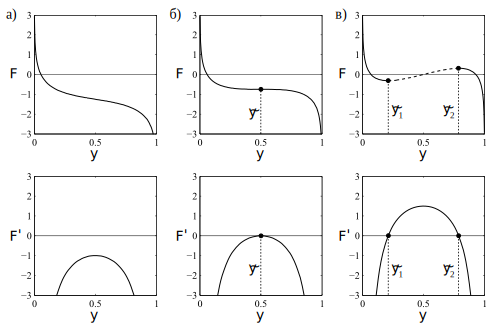
\includegraphics[width=1.0\textwidth]{analysis_sigm_stability}}
        \caption{Интервалы устойчивости решений системы~\eqref{eq:simple_microensemble_model}, определяемые знаком функции $F^{\prime}(\scalar{y})$, в случае: а)~$0,25 < \mu \theta / \alpha$; б)~$0,25 = \mu \theta / \alpha$; в)~$0,25 > \mu \theta / \alpha$ (участки графика с устойчивыми и неустойчивыми решениями обозначены соответственно сплошной и пунктирной линиями).}
        \label{fig:analysis_sigm_stability}
    \end{minipage}
\end{figure}

Отметим, что включение точки $\scalar{y}^{\sim}$ в область устойчивых решений при $d = 0$, так же как и выключение точек $\left\{\scalar{y}^{+}, \scalar{y}^{-}\right\}$ при $d > 0$, можно определить, рассмотрев их на графиках решения. В первом случае (\seefigure~\ref{fig:analysis_sigm_bound_points}а) устойчивость точки равновесия $\scalar{y}^{*} = \scalar{y}^{\sim}$ является результатом того, что в её окрестности градиент $\nabla\scalar{y}$, пропорциональный по величине и знаку $F(\scalar{y})$, будет направлять траекторию системы к ней, хотя скорость сходимости при этом будет крайне медленной в виду пологости функции $F(\scalar{y})$ в окрестности точки $\scalar{y}^{\sim}$. Во втором случае (\seefigure~\ref{fig:analysis_sigm_bound_points}б) в правой полуокрестности точки равновесия $\scalar{y}^{*} = \scalar{y}^{+}$ градиент $\nabla\scalar{y}$ уводит траекторию системы от неё, а в левой полуокрестности --- направляет к ней, но при условии, что величина градиента не позволит значению переменной $\scalar{y}$ оказаться в области $\left(\scalar{y}^{+}; 1\right]$, иначе градиент снова будет уводить траекторию от данной точки равновесия. Для точки $\scalar{y}^{*} = \scalar{y}^{-}$ ситуация симметрична, поэтому в дальнейшем без потери общности в рассуждениях мы будем подразумевать неустойчивость решений $\scalar{y}^{*} = \left\{\scalar{y}^{+}, \scalar{y}^{-}\right\}$.

\begin{figure}[ht]
    \begin{minipage}{\textwidth}
        \makebox[\textwidth][c]{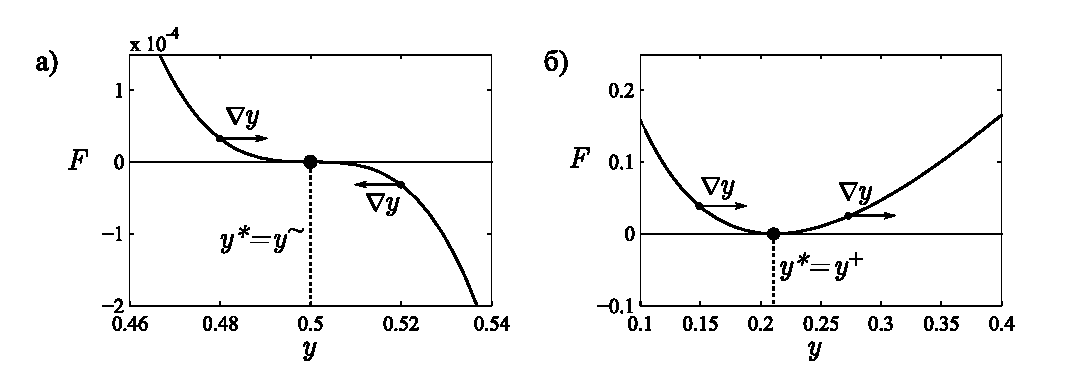
\includegraphics[width=1.0\textwidth]{analysis_sigm_bound_points}}
        \caption{Определение устойчивости пограничных точек $\scalar{y}^{\sim}$ и $\scalar{y}^{+}$, для которых $F^{\prime}(\scalar{y}) = 0$, по градиенту $\nabla\scalar{y}$ в точках их окрестности.} 
        \label{fig:analysis_sigm_bound_points}
    \end{minipage}
\end{figure}

\subsubsection{Бифуркационный анализ}

Основываясь на решении~\eqref{eq:sigm_stability_bounds_y}, можно определить важные свойства модели с точки зрения бифуркационного анализа. Однако прежде отметим вхождение в это решение отношения $\theta/\alpha$ --- параметр $\theta$ будем рассматривать как модулирующий коэффициент, поскольку значение параметра $\alpha$ задаёт изначальную (фиксированную) бифуркационную конфигурацию модели, которая затем в процессе функционирования будет меняться в соответствии с текущим значением параметра $\theta$. Поэтому в первую очередь мы рассмотрим влияние на модель параметра $\alpha$, а уже затем параметра $\theta$.

Как показано \onfigure~\ref{fig:analysis_sigm_bifurcations}а, в модели наблюдается бифуркация типа суперкритическая \inquotes{вилка}: при монотонном возрастании значения параметра $\alpha$ точка устойчивого равновесия преобразуется в точку неустойчивого равновесия, порождая при этом две новых устойчивых точки (\onfigure~\ref{fig:analysis_sigm_bifurcations}в пунктиром обозначены соответствующие при этом значения параметра $i$, обеспечивающие симметрию \inquotes{вилки}). Это происходит благодаря тому, что кривая решений $F(\scalar{y})$ теряет монотонность и приобретает $s$-образную складку (\seefigure~\ref{fig:analysis_sigm_stability}в) --- в этом случае точка бифуркации соответствует условию возникновения двух вещественных корней в~\eqref{eq:sigm_stability_bounds_y}, которое определяется равенством $0,25 - \mu \theta / \alpha = 0$. Таким образом, точкой бифуркации будет:
\begin{equation}
    \label{eq:sigm_bifurcation_alpha}
    \alpha =  4 \mu \theta.
\end{equation}

\begin{figure}[ht]
    \makebox[\textwidth][c]{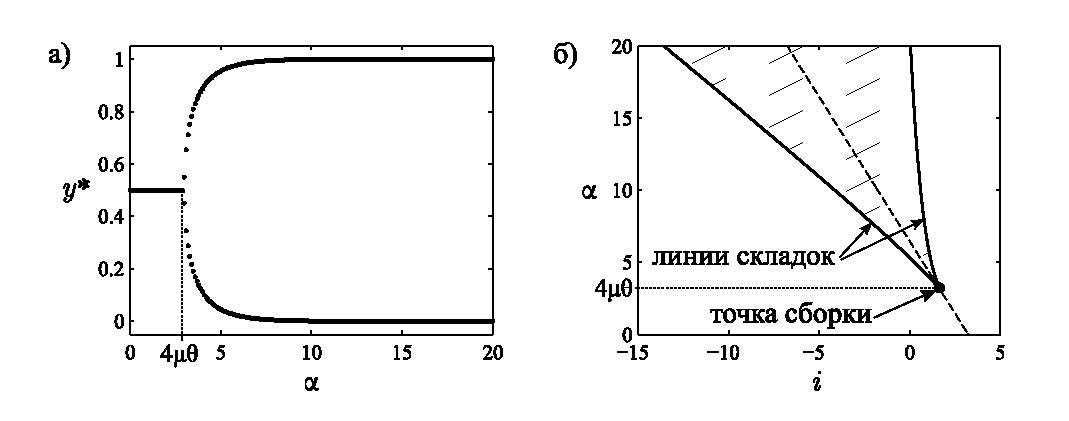
\includegraphics[width=1.0\textwidth]{analysis_sigm_bifurcations}}
    \makebox[\textwidth][c]{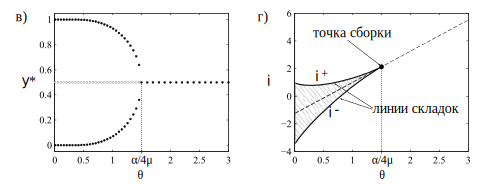
\includegraphics[width=1.0\textwidth]{analysis_sigm_bifurcations_p2}}
    \caption{Бифуркационные диаграммы: а-б) бифуркация типа суперкритическая \inquotes{вилка} (закрашенные круги соответствуют точкам устойчивого равновесия, проколотые -- неустойчивого); в-г) бифуркация типа \inquotes{сборка} (би-стабильная область заштрихована, уни-стабильная -- нет).}
    \label{fig:analysis_sigm_bifurcations}
\end{figure}

Как было отмечено ранее, при наличии $s$-образной складки в графике функции $F(\scalar{y})$ система~\eqref{eq:simple_microensemble_model} в зависимости от значения параметра $i$ может иметь одно или два устойчивых состояния, что хорошо видно \onfigure~\ref{fig:analysis_sigm_equilibriums}б. С учётом выражения~\eqref{eq:graphic_solution} и того, что корни~\eqref{eq:sigm_stability_bounds_y} соответстуют точкам перегиба функции $F(\scalar{y})$, очевидным образом вытекает условие существования режима с двумя устойчивыми состояниями: $i \in \left(i^{-}; i^{+}\right)$ при $\alpha > 4 \mu \theta$, где:
\begin{equation}
    \label{eq:sigm_stability_bounds_i}
    \begin{alignedat}{2}
        i^{\mp} &= -\alpha \scalar{y}^{\mp} + \mu \theta g_{\sigma}^{-1}(\scalar{y}^{\mp}) = \\
                &= -\alpha \left(0,5 \pm \sqrt{0,25 - \mu \theta / \alpha}\right) + \mu \theta \left(3 + \ln\dfrac{0,5 \pm \sqrt{0,25 - \mu \theta / \alpha}}{0,5 \mp \sqrt{0,25 - \mu \theta / \alpha}}\right).
    \end{alignedat}
\end{equation}

Таким образом, при монотонном возрастании значения параметра $i$ в точке $i^{-}$ возникает дополнительная пара из точек неустойчивого и устойчивого равновесия в дополнение к уже существующей устойчивой (\onfigure~\ref{fig:analysis_sigm_equilibriums}в точки $\scalar{y}^{*}_{2}$, $\scalar{y}^{*}_{3}$ и $\scalar{y}^{*}_{1}$ соответственно), а в точке $i^{+}$ изначально существовавшая точка аннигилируется вместе с точкой неустойчивого равновесия, в результате чего в системе вновь будет существовать единственное и устойчивое решение -- аналогично и в обратную сторону.

Данная ситуация соответствует бифуркации типа \inquotes{сборка}, которая изображена \onfigure~\ref{fig:analysis_sigm_solution_surface}а в виде зависящей от параметров $\scalar{i}$ и $\alpha$ поверхности решений системы~\eqref{eq:simple_microensemble_model} согласно выражению~\eqref{eq:graphic_solution}. Для наглядности \onfigure~\ref{fig:model_sigm_configurations} показаны различные срезы этой поверхности, привязанные к плоскости параметров. Сама же плоскость параметров более детально изображена на \onfigure~\ref{fig:analysis_sigm_bifurcations}в, где демонстрируется зависимость точек бифуркации $i^{-}$ и $i^{+}$ от значений параметра $\alpha$. 
\begin{figure}[ht]
    \makebox[\textwidth][c]{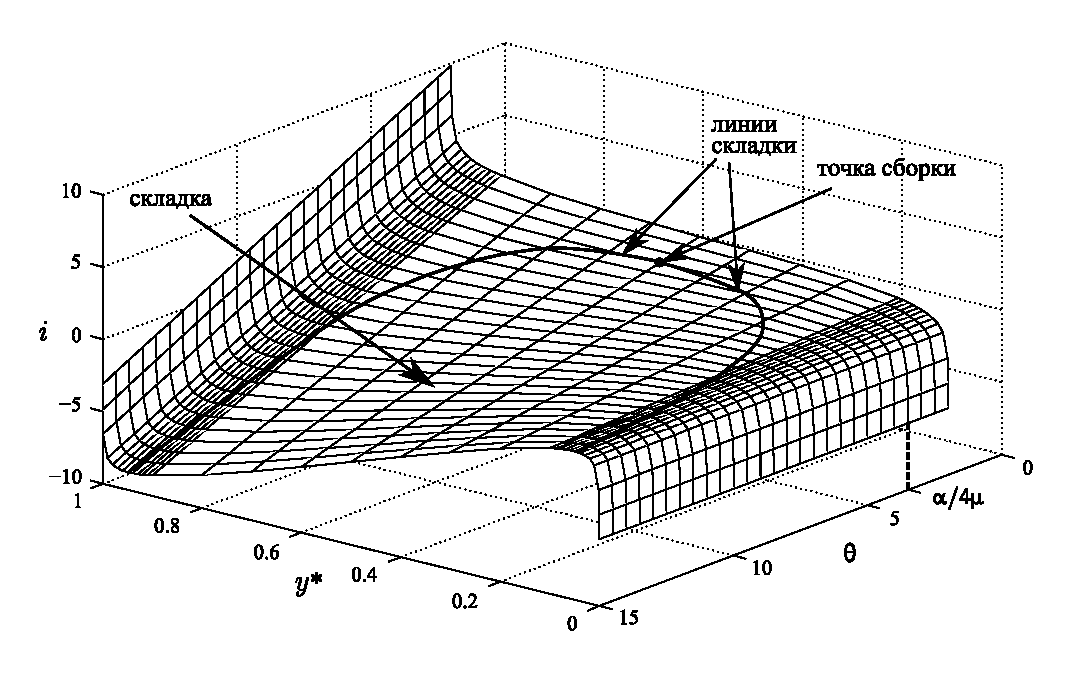
\includegraphics[width=0.95\textwidth]{analysis_sigm_solution_surface}}
    \makebox[\textwidth][c]{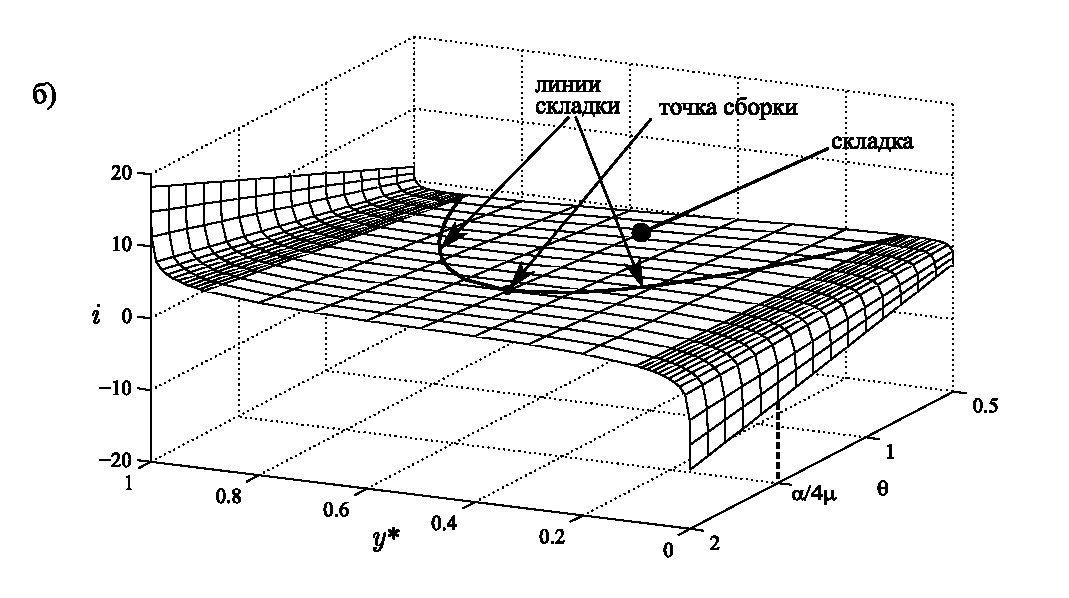
\includegraphics[width=0.95\textwidth]{analysis_sigm_solution_surface_p2}}
    \caption{Поверхность решений системы~\eqref{eq:simple_microensemble_model}, построенная по параметрам: а) $\alpha$ и $\scalar{i}$ при $\theta = 1, \mu = 0,75$; б) $\theta$ и $\scalar{i}$ при $\alpha = 4,5, \mu = 0,75$.}
    \label{fig:analysis_sigm_solution_surface}
\end{figure}
При этом \socalled точка сборки, определяющая точку возникновения $s$-образной складки, определяется равенством~\eqref{eq:sigm_bifurcation_alpha} и с учётом выражения~\eqref{eq:sigm_stability_bounds_i} равна:
\begin{equation}
    \nonumber
    \left(\alpha = 4 \mu \theta; \scalar{i} = \mu \theta\right).
\end{equation}

Как отмечалось выше, параметр $\theta$ входит в решение~\eqref{eq:sigm_stability_bounds_y} обратно пропорционально параметру $\alpha$, поэтому для него справедливы аналогичные результаты. Бифуркация типа суперкритическая \inquotes{вилка} продемонстрирована \onfigure~\ref{fig:analysis_sigm_bifurcations}б: при монотонном возрастании значения параметра $\theta$ две точки устойчивого равновесия сливаются вместе с точкой неустойчивого равновесия, образуя при этом одну устойчивую точку (\onfigure~\ref{fig:analysis_sigm_bifurcations}г пунктиром обозначены соответствующие при этом значения параметра $i$, обеспечивающие симметрию \inquotes{вилки}). Точка бифуркации находится из тех же соображений, что и~\eqref{eq:sigm_bifurcation_alpha}:
\begin{equation}
    \label{eq:sigm_bifurcation_theta}
    \theta =  \alpha / 4 \mu.
\end{equation}

Бифуркация типа \inquotes{сборка}, так же как и случае с параметром $\alpha$, изображена в виде поверхности решений системы~\eqref{eq:simple_microensemble_model}  \onfigure~\ref{fig:analysis_sigm_solution_surface}б, которая зависит от параметров $\scalar{i}$ и $\theta$: пара из точек устойчивого и неустойчивого равновесия возникает при пересечении линий складки, которые соответствуют значениям $i^{-}$ и $i^{+}$, в сторону области складки, а в при обратном направлении --- аннигилируется. Зависимость точек бифуркаций $i^{-}$ и $i^{+}$ от значений параметра $\theta$ продемонстрирована \onfigure~\ref{fig:analysis_sigm_bifurcations}г, а точка сборки, исходя из равенства~\eqref{eq:sigm_bifurcation_theta} и выражения~\eqref{eq:sigm_stability_bounds_i}, равна:
\begin{equation}
    \label{eq:sigm_bifurcation_theta_and_i}
    \left(\theta = \alpha / 4 \mu; \scalar{i} = \alpha / 4\right).
\end{equation}

\subsubsection{Дополнительные замечания}

Несмотря на то, что параметры $\alpha$ и $\theta$ вносят пропорциональный вклад в корни $y^{+}$ и $y^{-}$, которые зависят исключительно от величины $\mu \theta / \alpha$, их влияние на значения бифуркационных точек $i^{+}$ и $i^{-}$ имеет более сложный характер, что графически изображено \onfigure~\ref{fig:analysis_sigm_params_dependency}, а так же можно наблюдать \onfigure~\ref{fig:analysis_sigm_bifurcations}в-г. Имея в виду, что $\theta > 0$ по определению~\eqref{eq:full_single_neuron_model}, и учитывая точку бифуркации~\ref{eq:sigm_bifurcation_theta_and_i}, отметим следующее:
\begin{equation}
    \nonumber
    \begin{cases}
        \lim_{\theta \to +0} i^{+} &= 0 \\
        \lim_{\theta \to +0} i^{-} &= -\alpha 
    \end{cases}
    \quad
    \text{ и }
    \quad
    \begin{cases}
        \lim_{\theta \to \sfrac{\alpha}{4\mu} - 0} i^{+} &= \alpha / 4 \\
        \lim_{\theta \to \sfrac{\alpha}{4\mu} - 0} i^{-} &= \alpha / 4
    \end{cases}.
\end{equation}

\IncludeFigure[t]{analysis_sigm_params_dependency}{Зависящие от параметров $\alpha$ и $\theta$ поверхности точек бифуркации $i^{-}$ и $i^{+}$, проекции которых на плоскости $\left(\alpha,\scalar{i}\right)$ и $\left(\theta,\scalar{i}\right)$ изображены \onfigure~\ref{fig:analysis_sigm_bifurcations}в-г.}

Таким образом, если представить, что точки $i^{-}$ и $i^{+}$ задаются параметрическими функциями $i^{-}(z)$ и $i^{+}(z)$ с параметром $z \in \left[z_{0}; z_{1}\right]$, то $\theta$ будет определять значение параметра $z$, а $\alpha$ --- значения функций на концах интервала области определения, \ie значения $i^{-}(z_{0})$ и $i^{+}(z_{1})$. Более того, мы можем приблизить эти параметрические функции полиномом, представив выражение~\eqref{eq:sigm_stability_bounds_i} следующим образом:
\begin{equation}
    \nonumber
    i^{\mp}(z) = \alpha \left(-(0,5 \pm 0,5z) + \left(0,25 - 0,25z^2\right) \left(3 + \ln\left(\dfrac{1 \pm z}{1 \mp z}\right)\right)\right),
\end{equation}
где $z(\theta) = 2 \sqrt{0,25 - \mu\theta/\alpha}$, причём $z \in \left(0;1\right)$ при $\theta \in \left(\alpha/4\mu;0\right)$. Тогда применяя к функции логарифма разложение в ряд Тейлора в окрестности нуля, мы получим следующее:
\begin{align*}
    i^{\mp}(z) &= \alpha \left( -(0,5 \pm 0,5z) + \left(0,25 - 0,25z^2\right) \left(3 \pm 2\sum_{n=0}^{\infty}\dfrac{z^{2n+1}}{2n+1}\right) \right) = \\
               &= 0,25 \alpha \left( 1 \mp 2z - 3z^2 \pm 2 \left(1 - z^2\right) \sum_{n=0}^{\infty}\dfrac{z^{2n+1}}{2n+1} \right) = \\
               &= 0,25 \alpha \left( 1 \mp 2z - 3z^2 \pm 2\left(z + \sum_{n=1}^{\infty}\dfrac{z^{2n+1}}{2n+1} - \sum_{n=0}^{\infty}\dfrac{z^{2n+3}}{2n+1}\right)\ \right).
\end{align*}
После перенумерации первой суммы так, чтобы индекс начинался с нуля, и сложения коэффициентов при одинаковых степенях получим окончательное выражение в виде:
\begin{equation}
    i^{\mp}(z) = 0,25 \alpha \left( 1 - 3z^2 \mp 4 \sum_{n=0}^{\infty}\dfrac{z^{2n+3}}{(2n+3)(2n+1)} \right),
\end{equation}
которое позволяет оценить характер изменения величин $i^{-}$ и $i^{+}$, а так же позволяет определить монотонность убывания величины $\Delta i(z) = i^{+}(z) - i^{-}(z)$ при возрастании значении $\theta$.
% лежит в треугольнике

%\begin{Statement}
%    \todo{про мягкий режим и условия его существования.}
%\end{Statement}
%
%\begin{Statement}
%    \todo{про жёсткий режим и условия его существования.}
%\end{Statement}
%

%==============================================================================
\subsection{Модель с оригинальной функцией активации}  \label{subsection:analysis_origin}

Теперь рассмотрим вариант с использованием \textit{оригинальной} функции активации. На рисунке~\ref{fig:analysis_origin_equilibriums} приведены графические решения согласно выражению~\eqref{eq:graphic_solution} и соответствующие графики функции $F(\scalar{y})$ согласно выражению~\eqref{eq:functional_y} для следующих наборов значений параметров: а) $\alpha = 0  $ и $i =  2   $; б) $\alpha = 0,5$ и $i =  0,95$; в) $\alpha = 2,5$ и $i =  2   $; г) $\alpha = 5,5$ и $i =  0,5 $; д) $\alpha = 60 $ и $i = -20$, а значения  $\mu = 0,75$, $\theta = 1$, $p = 1,0$ -- одинаковы для всех вариантов. Можно заметить, учитывая результаты анализа из~\autoref{subsection:analysis_sigm}, что основные отличия от модели с \textit{сигмоидальной} функцией активации будут следствием наличия не одной, а двух взаимодействующих $s$-образных складок в графике решений, которые дают большее разнообразие режимов функционирования (\seefigure~\ref{fig:analysis_origin_equilibriums}):
\begin{itemize}
    \item[а)] Кривая решений не имеет складок: система имеет ровно одну точку устойчивого равновесия, так же как и в случае с \textit{сигмоидальной} функцией активации.
    \item[б)] Возникает первая складка: в системе появляется область би-стабильности, соответствующая интервалу $\scalar{i} \in (i_{low}^{-}; i_{low}^{+})$.
    \item[в)] Возникает вторая складка: область би-стабильности системы дополняется интервалом $\scalar{i} \in (i_{high}^{-}; i_{high}^{+})$.
    \item[г)] Происходит наложение складок: в системе возникает область три-стабильности на пересечении интервалов би-стабильности, \ie при $\scalar{i} \in (i_{low}^{-}; i_{low}^{+}) \cap (i_{high}^{-}; i_{high}^{+})$.
    \item[д)] Происходит исчезновение первой складки: в системе остаётся единственная область би-стабильности, соответствующая $\scalar{i} \in (i_{high}^{-}; i_{high}^{+})$.
\end{itemize}
\IncludeFigure[p]{analysis_origin_equilibriums}{Графическое решение системы~\eqref{eq:simple_microensemble_model} и график функции $F(\scalar{y})$ для случаев: а) отсутствия складок; б) наличия только первой складки; в) наличия двух неперекрывающихся складок; г) наличия двух перекрывающихся складок; д) наличия только второй складки.}

\subsubsection{Анализ устойчивости точек равновесия}

Как и в~\autoref{subsection:analysis_sigm}, для определения интервалов устойчивости-неустойчивости точек равновесия $\scalar{y}^{*}$ необходимо решить равенство $F^{\prime}(\scalar{y}) = 0$, которое в соответствии с определением функции $g^{-1}_{s}$~\eqref{eq:unactivation_function_original} примет вид:
\begin{equation}
\nonumber
    F^{\prime}(\scalar{y}) = \dfrac{d}{d\scalar{y}}\left( \alpha \scalar{y} + \scalar{i} - \mu \theta g^{-1}(\scalar{y}) \right) = 
    \begin{cases}
        \alpha - \dfrac{312 \mu \theta \scalar{x}}{(\scalar{x} + 1)^{2}} = 0,   & \scalar{x} \in \left(x_{01}; x_{12}\right] \\
        \alpha - \dfrac{z_{12} \mu \theta}{(\scalar{y} - 1)^{2}} = 0,           & \scalar{y} \in \left(y_{12}; 1\right] \\
    \end{cases}
\end{equation}
где $\scalar{x} = e^{-120 \cdot (\scalar{y} - 0,1935)}$, а $x_{01} = e^{120 \cdot 0,1935} \approx 1,2 \cdot 10^{10}$ и $x_{12} = e^{-120 \cdot (y_{12} - 0,1935)} \approx 2,1 \cdot 10^{-3}$. При этом обратное преобразование определено как $\scalar{y} = 0,1935 - \ln(\scalar{x}) / 120$.

Так же сразу отметим, что исходя из определения функции $g^{-1}_{s}$ в точке $\scalar{y} = 0$, $F^{\prime}(0) = -\infty$ и поэтому точка равновесия $\scalar{y}^{*} = 0$ всегда устойчива и существует при $\scalar{i} < \mu \theta u_{01}$ --- обозначим это решение как $y_{low}^{+}$.

Для решения полученных равенств приведём их к виду квадратных уравнений. Для этого, во-первых, примем во внимание, что переменная $\scalar{y}$ в системе~\eqref{eq:simple_microensemble_model} достигает значения 1 лишь в пределе, что обусловлено свойством \textit{оригинальной} функции активации: $\scalar{y} = \lim_{\scalar{u} \to \infty} f(\scalar{u}, \theta) = 1$. Во-вторых, отметим, что при $\alpha = 0$ решений не существует и $F^{\prime}(\scalar{y}) < 0\ \forall \scalar{y}$ --- однако это условие в дальнейшем войдёт в более общее условие устойчивости, поэтому отдельно оно рассматриваться не будет. Таким образом, после деления равенств на $\alpha$ и домножения соответственно на $(\scalar{x} + 1)^{2}$ и $(\scalar{y} - 1)^{2}$ мы получим следующие квадратные уравнения:
\begin{equation}
    \nonumber
    \begin{cases}
        \scalar{x}^{2} + \left( 2 - 312 \mu \theta / \alpha \right) \scalar{x} + 1 = 0,     & \scalar{x} \in \left(x_{01}; x_{12}\right] \\
        \scalar{y}^{2} - 2 \scalar{y} + \left( 1 - z_{12} \mu \theta / \alpha \right) = 0,  & \scalar{y} \in \left(y_{12}; 1\right] \\
    \end{cases}
\end{equation}
решением которых будут корни:
\begin{equation}
    \begin{cases}
        \scalar{x}_{1,2} = \left( 156 \mu \theta / \alpha - 1\right) \pm \sqrt{\left( 156 \mu \theta / \alpha - 1\right)^{2} - 1}, & \scalar{x} \in \left(x_{01}; x_{12}\right] \\
        \scalar{y}_{3\phantom{,4}}   = 1 - \sqrt{z_{12} \mu \theta / \alpha},                                                      & \scalar{y} \in \left(y_{12}; 1\right] \\
    \end{cases}
\end{equation}
где корень $\scalar{y}_{4} = 1 + \sqrt{z_{12} \mu \theta / \alpha}$ не рассматривается, т.к. при любых допустимых значениях параметров величина $\scalar{y}_{4} > 1$, \ie не принадлежит области определения переменной $\scalar{y}$. 

Так как существование каждого из корней ограничено определённым интервалом значений и, кроме того, в решении $\scalar{x}_{1,2}$ выражение под знаком корня может принимать отрицательные значения, необходимо рассмотреть их подробнее. Для этого обозначим как $y_{low}^{-} = \scalar{y}_{1} = 0,1935 - \ln(\scalar{x}_{1})/120$ и $y_{high}^{+} = \scalar{y}_{2} = 0,1935 - \ln(\scalar{x}_{2})/120$ для случая, когда $\scalar{x}_{1,2}$ --- два различных вещественных значения (подразумевая, что $\scalar{x}_{1} > \scalar{x}_{2}$), а так же $y_{high}^{-} = \scalar{y}_{3}$. При этом доказательства включения или выключения граничных точек интервалов устойчивости, где $F^{\prime}(\scalar{y}) = 0$, рассматриваться не будет, т.к. является очевидным следствием того же принципа, который использовался в аналогичном подразделе~\autoref{subsection:analysis_sigm}. Таким образом, обозначив через $d = \left( 156 \mu \theta / \alpha - 1\right)^{2} - 1$, мы получим следующее:
\begin{enumerate}[wide]
    \item Если $d < 0$, то корни $\scalar{y}_{1,2}$ представляют собой пару комплексно-сопряжённых чисел и $\forall\scalar{y} \in \left(0; y_{12}\right]\ F^{\prime}(\scalar{y}) > 0$. Кроме того, в этом случае $\mu \theta / \alpha < 1 / 78$ и, как следствие, $\scalar{y}_{3} \in (1 - \sqrt{z_{12} / 78}; 1] \subset (y_{12}; 1]$, \ie лежит в интервале допустимых значений. Поэтому область устойчивых решений определяется множеством точек $\{0\} \cup (y_{high}^{-}; 1]$, на котором $F^{\prime}(\scalar{y}) < 0$, как показано \onfigure~\ref{fig:analysis_origin_stability}в.
    \item Если $d = 0$, то корни $\scalar{y}_{1,2}$ обратятся в константу $\scalar{y} = 0,1935$, которая соответствует точке неустойчивого равновесия. Поэтому область устойчивых решений совпадает со случаем, когда $d < 0$.
    \item Если $d > 0$, то все три корня $\scalar{y}_{1,2,3}$ являются действительными числами, однако условия их существования в этом случае зависят от значений параметров --- подробнее этот вопрос освещён далее. Здесь же можно отметить, что для корней $\scalar{y}_{2}$ и $\scalar{y}_{3}$ условие существования одинаково и включает в себя условие существования корня $\scalar{y}_{1}$, но не наоборот. Поэтому область устойчивых решений будет определяться одним из трёх множеств, на которых $F^{\prime}(\scalar{y}) < 0$: $[0; 1]$ (\seefigure~\ref{fig:analysis_origin_stability}а), $\{0\} \cup (y_{low}^{-}; 1]$ или $\{0\} \cup (y_{low}^{-}; y_{high}^{+}) \cup (y_{high}^{-}; 1]$ (\seefigure~\ref{fig:analysis_origin_stability}б).
    % $\scalar{x}_{1,2} \sim O(2d)$
\end{enumerate}
\begin{figure}[ht]
    \begin{minipage}{\textwidth}
        \makebox[\textwidth][c]{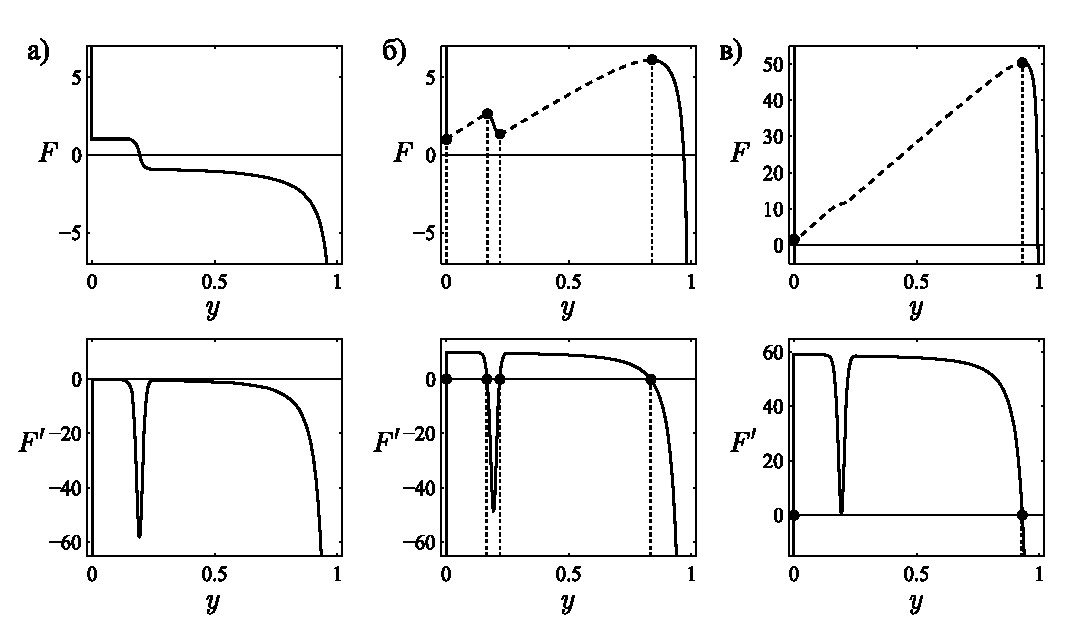
\includegraphics[width=1.0\textwidth]{analysis_origin_stability}}
        \caption{Интервалы устойчивости решений системы~\eqref{eq:simple_microensemble_model}, определяемые знаком функции $F^{\prime}(\scalar{y})$, в случае: а)~...; б)~...; в)~... (участки графика с устойчивыми и неустойчивыми решениями обозначены соответственно сплошной и пунктирной линиями).}
        \label{fig:analysis_origin_stability}
    \end{minipage}
\end{figure}

\subsubsection{Бифуркационный анализ}


%==============================================================================
%                       Характерные свойства и динамика
%==============================================================================
\newpage
\section{Характерные свойства и динамика} \label{section:neuron_dynamic}

Стоит отметить, что несмотря на отсутствие точного аналитического решения системы~\eqref{eq:simple_microensemble_model}, найденные бифуркационные точки позволяют не только подобрать фиксированные параметры модели $\mu$ и $\alpha$ (в нормализованных условиях, когда значение управляющего параметра $\theta = 1$), но и оценить вносимые при вариации значений параметра $\theta$ изменения в модели с точки зрения нейросетевой обработки информации.

%==============================================================================
\subsection{Определения и свойства}

%==============================================================================
\subsection{Численное моделирование}

Для выполнения численных экспериментов с рабочей моделью необходимо в первую очередь привести её к эквивалентной дискретной форме, применив один из разностных методов. Для этого в ходе исследований было рассмотрено применение классических методов, таких как явный метод Эйлера, модифицированный метод Эйлера с пересчётом (разновидность метода Рунге-Кутты второго порядка точности), а так же явный метод Рунге-Кутты четвёртого порядка точности~\cite{Hairer1990}. Более подробно этот вопрос освещён \inappendix~\ref{appendix:differential_schemes_compare}. Здесь же отметим, что при выборе разумного с точки зрения точности и вычислительной эффективности шага $h$ использование того или иного метода не вносило существенных изменений в результаты численных экспериментов. Поэтому описанные далее в главе результаты подразумевают применение явного метода Эйлера с шагом $h = 0,01$:
\begin{equation*}
    \begin{cases}
        \scalar{u^{t+1}} = \scalar{u^{t}} + h \times ( \alpha\scalar{y^{t}} + \scalar{i^{t}} - \scalar{p^{t}} - \mu\scalar{u^{t}} ), \\ 
        \scalar{y^{t+1}} = f(\scalar{u^{t+1}}, \theta).
    \end{cases}
\end{equation*}


%==============================================================================
%               Моделирование простейшей нейронной сети
%==============================================================================
\section{Моделирование простейших нейронных структур} \label{section:neuron_modeling}

Для проверки принципиальной работоспособности предлагаемой модели далее будут рассмотрены две задачи: задача анализа независимых компонент (\acr{ICA}) и задача построения нейросетевого детерминированного конечного автомата (\acr{FSM}). Для их решения будут смоделированы простые нейронные сети с применением микроансамблей в качестве элементарных элементов. При этом для решения первой задачи параметры модели будут соответствовать <<мягкому>> режиму работы, чтобы продемонстрировать\todo{...}  При решении второй задачи параметры модели будут соответствовать <<жёсткому>> режиму, демонстрируя\todo{...}

%%==============================================================================
%\subsection{Решение задачи анализа независимых компонент}
%
%Задача анализа независимых компонент, более подробная постановка которой изложена в Приложении~\ref{appendix:ica_description}, имеет важное прикладное значение, будучи связанной с решением таких проблем, как слепое разделение сигналов и снижение размерности данных~\cite{Hyvarinen2004}. Мы рассмотрим решение частной задачи \acr{ICA} --- <<F{\"o}ldiak bars>>~\cite{Foldiak1990}, которая часто используется в нейросетевой области для первичной проверки соответствующих моделей.
%
%Входные данные представляют собой бинарные изображения размером $8\,\times\,8$ пикселей, сгенерированные с использованием 16-ти независимых компонент: 8-ми горизонтальных и 8-ми вертикальных линий, каждая из которых появлятся на изображении с вероятностью $1/8$ --- независимые компоненты и примеры получаемых на их основе изображений представлены \onfigure~\ref{img:ica_patterns}. Решение же задачи заключается, во-первых, в нахождении в процессе обучения независимых компонент, использованных при генерации изображений, и во-вторых, в разложении в процессе штатной работы входных данных по найденным независимым компонентам. Другими словами, в результате обучения каждой независимой компоненте необходимо поставить в соответствие некоторый нейрон, активность которого будет отражать наличие этой компоненты во входном изображении.
%
%\begin{figure}[ht]
%    \makebox[\textwidth][c]{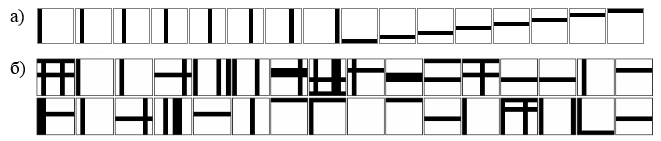
\includegraphics[width=1.0\textwidth]{ica_patterns}}
%    \caption{Бинарные изображения размером 8х8 пикселей: а) набор из 16-ти независимых компонент; б) примеры входных паттернов.}
%    \label{img:ica_patterns}
%\end{figure}
%
%Стоит отметить, что данная постановка задачи соответствует классу нелинейных задач, т.к. в точках пересечения горизонтальных и вертикальных линий происходит не обычная операция сложения значений $(x + y)$, а сложение значений по модулю: $(x + y) \bmod 1$ ---, что вносит нелинейные искажения в складываемые изображения линий.
%
%\subsubsection{Модель нейронной сети}
%
%Для решения данной задачи была реализована однослойная нейронная сеть, состоящая из 16-ти нейронов, что отражает наши априорные знания о числе ожидаемых независимых компонент в обрабатываемых данных. Формальная модель \acr{NN} имеет вид:
%\begin{equation}
%    \nonumber
%    \begin{cases}
%        \dot{\vector{u}} &= \left(\alpha \matrix{I} - \matrix{V} \right)^{\top} \vector{y} + \matrix{W}^{\top} \vector{x} - \mu \vector{u},\\
%        \vector{y}       &= f(\vector{u}),
%    \end{cases}
%\end{equation}
%где $\vector{x}_{64 \times 1}$ --- входной вектор, представляющий собой линеаризованное по столбцам входное изображение, $\matrix{W}_{64 \times 16}$ --- как и ранее, матрица, отражающая возбуждающие связи от входного вектора к элементами сети, $\matrix{V}_{16 \times 16}$ --- матрица, отражающая тормозные связи между самими элементами сети. В соответствии с работой~\cite{Fyfe2007}, использование взаимных тормозных связей, обучаемых хэббо-подобным правилом, будет приводить к взаимной декорреляции выходов \acr{NN}. В качестве активационной функции была применена оригинальная функция $s$ (ХХХ) и использованы следующие значения параметров: $\mu = 0,75$, $\theta = 1$, $\alpha = (N - 1) \cdot \omega = 10 \cdot 0,25 = 2,5$ и $p = 1,01$.
%
%Для обучения как возбуждающих, так и тормозных связей использовался один из вариантов STDP-правила~\cite{Izhikevich2003} (\todo{ЗАМЕНИТЬ НА ОБЫЧНОЕ ХЭББОВСКОЕ ПРАВИЛО}):
%\begin{equation}
%    \nonumber
%    \begin{cases}
%        \Delta_{ji} &= 
%        \begin{cases}
%            \vector{y}_{j} \vector{y}_{i} \left( \dfrac{A_{E}}{1/\tau_{E} + \vector{y}_{i}} + \dfrac{A_{I}}{1/\tau_{I} + \vector{y}_{i}}\right), &\text{ если } i \ne j \\
%            0, &\text{ иначе } \\
%        \end{cases} \\
%        \vector{w}_{ji} &= \max \left( 0, \vector{w}_{ji} + \beta_{\vector{w}} \Delta_{ji} \right), \\
%        \vector{v}_{ji} &= \max \left( 0, \vector{v}_{ji} - \beta_{\vector{v}} \Delta_{ji} \right), \\
%    \end{cases}
%\end{equation}
%где $A_{E} = 1,01$, $A_{I} = -0,58$, $\tau_{E} = 5$, $\tau_{I} = 38$, $\beta_{\vector{w}} = 0,001$, $\beta_{\vector{v}} = 0,01$, а функция $\max$ обеспечивает неотрицательность элементов матриц $\matrix{W}$ и $\matrix{V}$. Кроме того, после каждой итерации выполнялась нормализация весовых матриц по столбцам, так чтобы $\forall i\ \sum_{j}\vector{w}_{ji} = w^{total}$, где $w^{total} = 2,7$, и $\forall i\ \sum_{j}\vector{v}_{ji} = v^{total}$, где $v^{total} = 5,4$.
%
%\subsubsection{Результаты численных экспериментов}
%
%\begin{figure}[ht]
%    \makebox[\textwidth][c]{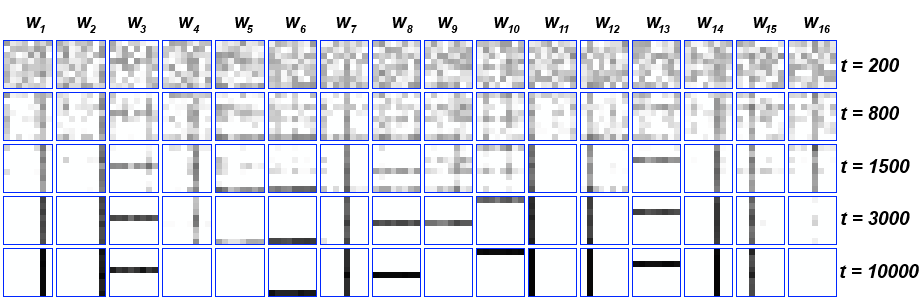
\includegraphics[width=1.0\textwidth]{ica_learning_weights}}
%    \caption{\todo{Изменение векторов-столбцов возбуждающей матрицы $\matrix{W}$ в процессе обучения...}}
%    \label{img:ica_learning_weights}
%\end{figure}
%
%\begin{figure}[ht]
%    \makebox[\textwidth][c]{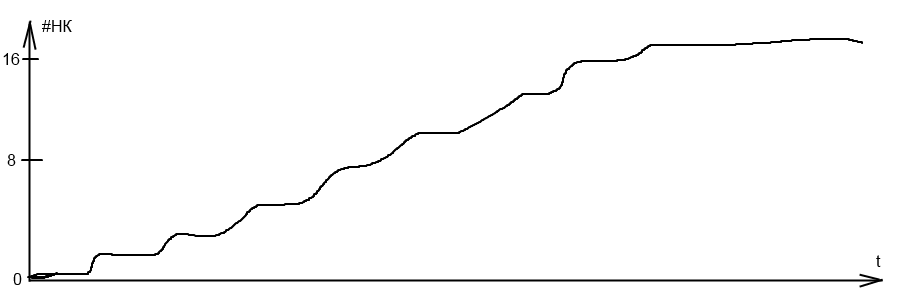
\includegraphics[width=1.0\textwidth]{ica_learning_progress}}
%    \caption{\todo{Количество найденных уникальных компонент в процессе обучения...}}
%    \label{img:ica_learning_progress}
%\end{figure}
%
%\begin{figure}[ht]
%    \makebox[\textwidth][c]{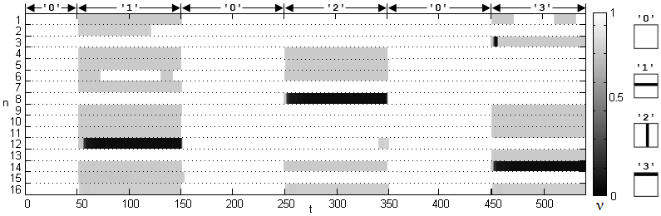
\includegraphics[width=1.0\textwidth]{ica_modeling_result}}
%    \caption{\todo{Результат моделирования...}}
%    \label{img:ica_modeling_result}
%\end{figure}


%==============================================================================
\subsection{Построение нейросетевого конечного автомата}

\todo{Вводная часть...}

\subsubsection{Модель нейронного конечного автомата}

Определим детерминированный конечный автомат (\acr{FSM})~\cite{Hopcroft2008} как формальную математическую структуру $M = \left( \usualset{A}, \usualset{S}, s_{0}, \delta \right)$, где $\usualset{A}$ --- конечное множество входных символов (входной алфавит), $\usualset{S}$ --- конечное множество состояний автомата, $s_{0} \in \usualset{S}$ --- начальное состояние автомата, $\delta\!: \usualset{S}\!\times\!\usualset{A} \to \usualset{S}$ --- функция перехода, отображающая упорядоченную пару элементов (состояние автомата и входной символ) в новое состояние автомата. Если мы обозначим через $q \in \usualset{S}$ текущее состояние автомата, которое в начальный момент времени совпадает с $s_{0}$, то функционирование автомата заключается в последовательном считывании символов $a_{i}$ из входной последовательности $\left\{ a_{0} a_{1} \ldots | a_{j} \in \usualset{A} \right\}$ и переходе в новое состояние: $q = \delta \left( q, a_{i} \right)$. Стоит отметить, что в структуру $M$ часто добавляют множество \socalled заключительных состояний $\usualset{F} \subseteq \usualset{S}$ для верификации считанной входной последовательности, однако в данной работе в этом нет необходимости.

Построение нейросетевой модели по заданной структуре \acr{FSM} можно разбить на две части: построение топологии сети и подбор весовых коэффициентов связей сети. Для задания топологии в первую очередь необходимо каждому элементу всех множеств структуры $M$ поставить в соответствие свой нейрон $n_{i}$: обозначим множество $\left\{ n_{k} | k = \usualset{A} \right\}$, соответствующее множеству $\usualset{A}$, как множество \inquotes{входных} нейронов, множество $\left\{ n_{k} | k = \usualset{S} \right\}$, соответствующее множеству $\usualset{S}$, как множество нейронов \inquotes{состояний} и множество $\left\{ n_{k} | k = D(\delta) \right\}$, соответствующее множеству $S\!\times\!A$ (исключая элементы, для которых отображение $\delta$ не определено), как множество нейронов \inquotes{переходов}. Таким образом, сеть будет состоять из $N = \left|\usualset{A}\right| + \left|\usualset{S}\right| + \left|D(\delta)\right|$ нейронов.

Далее каждому переходу, заданному как элемент множества $\{ \left( s_{i}, s_{j}, a_{k} \right) | \exists \delta\!: s_{i}\!\times\!a_{k} \to s_{j} \}$, необходимо поставить в соответствие набор связей между нейронами сети. Учтём, что в любой момент времени может считываться только один входной символ и должен быть активен только один нейрон \inquotes{состояния} (исключая периоды смены текущего состояния \acr{FSM}, которые связаны с инертностью системы). Поэтому переход из одного состояния в другое является результатом взаимодействия тех нейронов, которые непосредственно соответствуют данному переходому в структуре $M$, а активность остальных должна быть пренебрежимо мала. В результате такой локализации вычислений нейронные связи в сети можно представить в виде типизированного набора, соответствующего каждому переходу в \acr{FSM}: $\beta_{st}$ --- двунаправленная тормозная связь между $n_{s_{i}}$ и $n_{s_{j}}$, $\beta_{tr}$ --- тормозная связь от $n_{s_{i}\!\times\!a_{k}}$ к $n_{a_{k}}$, $\gamma_{st}$ --- возбуждающая связь от $n_{s_{i}}$ к $n_{s_{i}\!\times\!a_{k}}$, $\gamma_{tr}$ -- возбуждающая связь от $n_{s_{i}\!\times\!a_{k}}$ к $n_{s_{j}}$, $\gamma_{in}$ --- возбуждающая связь от $n_{a_{k}}$ к $n_{s_{i}\!\times\!a_{k}}$. \todo{Таким образом, матрица связей \acr{NN} будет имеет следующий вид: ...}

Значения весовых коэффициентов связей подбираются путём решения системы неравенст, описывающей требуемое от элементов сети поведение. Для произвольного перехода $s_{i}\!\times\!a_{k}~\to~s_{j}$ эти требования можно сформулировать следующим образом:. \todo{Формально это соответствует следующей системе уравнений:}

Данная схема позволяет построить для произволного \acr{FSM} функционально эквивалентную нейросетевую модель. Перед началом моделирования начальное состоние $S_{0}$ может быть задано явно, например, как одно из начальных условий: $\nu_{s_{0}} = \nu^{high}$.

Для наглядности \onfigure~\ref{img:fsm_example_topology}а изображена простейшая схема \acr{FSM} с $\usualset{A} = \{ a_{1}, a_{2} \}$, $\usualset{S} = \{ s_{1}, s_{2}, s_{3} \}$ и функцией $\delta$, определённой как $\{ s_{1}\!\times\!a_{1} \to s_{2}$, $s_{2}\!\times\!a_{1} \to s_{3}$, $s_{3}\!\times\!a_{2} \to s_{1} \}$. Результат применения описанного выше преобразования --- функционально эквивалентная \acr{NN}, изображённая \onfigure~\ref{img:fsm_example_topology}б (на рисунке также изображены рекуррентные связи нейронов $\alpha_{st}$ и $\alpha_{tr}$). Используя параметры сети \todo{параметры}, можно вычислить коэффициенты связей (\seefigure~\ref{img:fsm_example_weights}): \todo{коэффициенты}.

\begin{figure}[ht]
    \makebox[\textwidth][c]{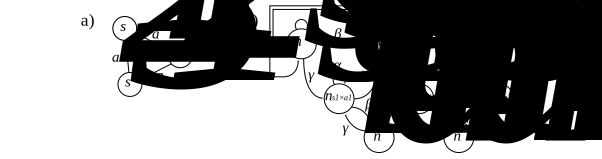
\includegraphics[width=1.0\textwidth]{fsm_example_topology}}
    \caption{Пример построения нейросетевого \acr{FSM}: а) диаграмма состояний автомата; б) эквивалентная диаграмме состояний схема \acr{NN}.} 
    \label{img:fsm_example_topology}  
\end{figure}

\begin{figure}[ht]
    \makebox[\textwidth][c]{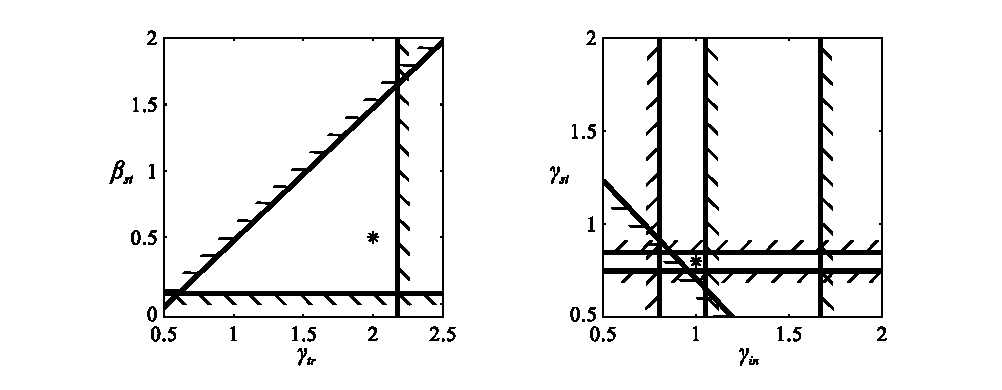
\includegraphics[width=1.2\textwidth]{fsm_example_weights}}
    \caption{Допустимые области значений для весовых коэффициентов, полученные при использовании параметров: \todo{значения параметров}. Ограничения обусловлены функциональными требованиями, наложенными на различные типы нейронов. } 
    \label{img:fsm_example_weights}  
\end{figure}


\subsubsection{Результаты численных экспериментов}

Результат моделирования простейшей схемы \acr{FSM} из предыдущего подраздела (\seefigure~\ref{img:fsm_example_topology}) представлен \onfigure~\ref{img:fsm_example_dynamic}, на котором отражена частота нейронов \inquotes{состояний} и периоды предъявления входных символов. Видно, что при подаче допустимых входных символов, \ie для которых определён переход из текущего состояния, происходит смена конфигурации: соответствующий текущему состоянию нейрон становится неактивным, а соответствующий новому состоянию --- активным. В то же время, при подаче недопустимого символа (интервал времени $[350; 375]$) состояние сети качественно остаётся без изменений. Кроме того, стоит отметить что непрерывное предъявление входного символа приводит к последовательной смене состояний до тех пор, пока схема автомата это допускает (интервал времени $[450; 500]$), что отражает периодичность происходящих в модели процессов.

\begin{figure}[ht]
    \makebox[\textwidth][c]{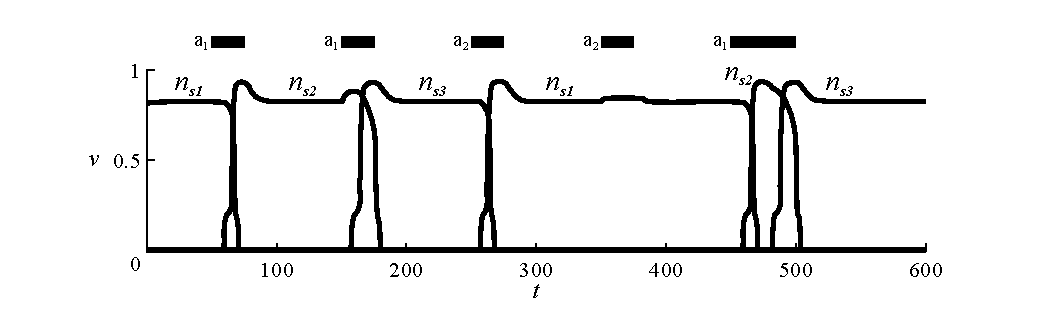
\includegraphics[width=1.1\textwidth]{fsm_example_dynamic}}
    \caption{Динамика нейронов \inquotes{состояний} нейросетевой модели \acr{FSM}, представленной \onfigure~\ref{img:fsm_example_topology}б. Верхние горизонтальные линии отражают временне периоды считывания входных символов.} 
    \label{img:fsm_example_dynamic}  
\end{figure}

Также работоспособность данного подхода проверялась и на более сложных примерах \acr{FSM}, один из которых приведён \onfigure~\ref{img:fsm_model_topology}, --- стоит отметить наличие в диаграмме состояний циклов и двойных переходов (наличие двойных дуг от одного состояния к другому). Как и ранее, в результате применения описанного выше преобразования была получена функционально эквивалентная нейросетевая модель со следующими параметрами: \todo{параметры}. Различные численные эксперименты, один из которых приведён \onfigure~\ref{img:fsm_model_dynamic}, показали, что нейросетевая модель автомата успешно обрабатывает любую последовательность входных символов, игнорируя недопустимые символы. При этом работоспособность сохраняется и при обработке достаточно длинных последовательностей (максимальная использованная длина последовательности составила 1000 символов) и при наличии больших временн\'{ы}х задержек между предъявлениями символов (максимальная использованная задержка составила порядка 10000 единиц), что подтверждает работоспособность данного подхода.

\begin{figure}[ht]
    \makebox[\textwidth][c]{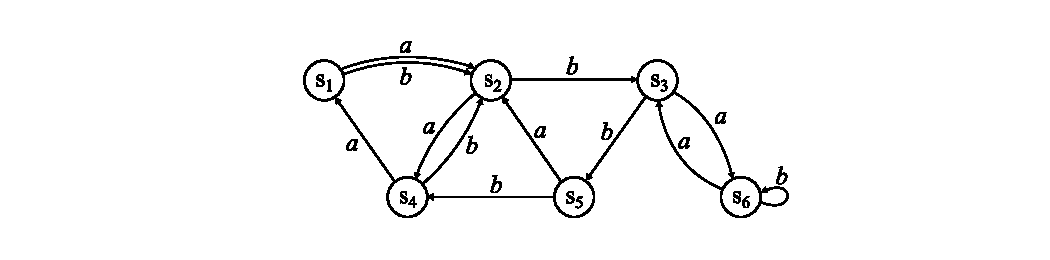
\includegraphics[width=1.2\textwidth]{fsm_model_topology}}
    \caption{Диаграмма состояний \acr{FSM}, использованного в процессе моделирования.}
    \label{img:fsm_model_topology}  
\end{figure}

\begin{figure}[ht]
    \makebox[\textwidth][c]{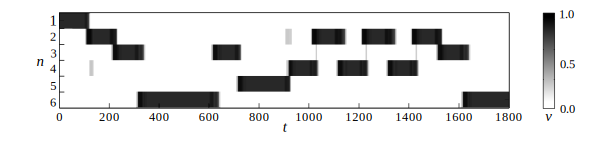
\includegraphics[width=1.1\textwidth]{fsm_model_dynamic}}
    \caption{Результаты численного моделирования нейросетевого \acr{FSM}, представленного \onfigure~\ref{img:fsm_model_topology}. Ось ординат соответствует индексам нейронов \inquotes{состояний}. Значение частоты нейронов выражено оттенками серого в соответствии со шкалой справа.} 
    \label{img:fsm_model_dynamic}  
\end{figure}

%==============================================================================
%                               Выводы по главе
%==============================================================================
\section{Выводы по главе \thechapter} \label{section:neuron_concls}



